\documentclass{article}
\usepackage[T1]{fontenc}
\usepackage{hyperref, amssymb, amsmath, graphicx, subfigure}

\setlength{\oddsidemargin}{.25in}
\setlength{\evensidemargin}{.25in}
\setlength{\textwidth}{6in}
\setlength{\topmargin}{-0.4in}
\setlength{\textheight}{8.5in}

\setlength{\parindent}{0in}
\setlength{\parskip}{8pt}

\newcommand{\heading}[6]{
  \renewcommand{\thepage}{#1-\arabic{page}}
  \noindent
  \begin{center}
  \framebox{
    \vbox{
      \hbox to 5.78in { \textbf{#2} \hfill #3 }
      \vspace{4mm}
      \hbox to 5.78in { {\Large \hfill #6  \hfill} }
      \vspace{2mm}
      \hbox to 5.78in { \textit{Instructor: #4 \hfill #5} }
    }
  }
  \end{center}
  \vspace*{4mm}
}

\newtheorem{theorem}{Theorem}
\newtheorem{definition}[theorem]{Definition}
\newtheorem{remark}[theorem]{Remark}
\newtheorem{lemma}[theorem]{Lemma}
\newtheorem{corollary}[theorem]{Corollary}
\newtheorem{proposition}[theorem]{Proposition}
\newtheorem{claim}[theorem]{Claim}
\newtheorem{observation}[theorem]{Observation}
\newtheorem{fact}[theorem]{Fact}
\newtheorem{assumption}[theorem]{Assumption}

\newenvironment{proof}{\noindent{\bf Proof:} \hspace*{1mm}}{
	\hspace*{\fill} $\Box$ }
\newenvironment{proof_of}[1]{\noindent {\bf Proof of #1:}
	\hspace*{1mm}}{\hspace*{\fill} $\Box$ }
\newenvironment{proof_claim}{\begin{quotation} \noindent}{
	\hspace*{\fill} $\diamond$ \end{quotation}}
	
\newcommand{\lecture}[4]{\heading{#1}{Probabilistic Proof Systems}{#2}{Alessandro Chiesa}{Scribe: #4}{#3}}



%%%%%%%%%%%%%%%%%%%%%%%%%%%%%%%%%%%%%%%%%%%%%%%%%%%%%%%%%%%%%%%%%%%%%%%%%%%%%%%
% PLEASE MODIFY THESE FIELDS AS APPROPRIATE:
\newcommand{\lecturenum}{1} % lecture number
\newcommand{\lecturedate}{\today} % date of lecture (e.g., 'March 20, 2010')
\newcommand{\lecturetitle}{IP\#1 - Graph Non-Isomorphism \& PSPACE Upper Bound} % lecture title
\newcommand{\scribename}{Shuangjun Zhang} % full name of scribe
% PUT HERE ANY PACKAGES, MACROS, etc., ADDED BY YOU
%
\usepackage{graphicx}
\usepackage{subfigure}
%%%%%%%%%%%%%%%%%%%%%%%%%%%%%%%%%%%%%%%%%%%%%%%%%%%%%%%%%%%%%%%%%%%%%%%%%%%%%%%


%%%%%%%%%%%%%%%%%%%%%%%%%%%%%%%%%%%%%%%%%%%%%%%%%%%%%%%%%%%%%%%%%%%%%%%%%%%%%%%
\begin{document}
\lecture{\lecturenum}{\lecturedate}{\lecturetitle}{\scribename}

\section{The class $\mathcal{NP}$}

The class $\mathcal{NP}$ can be regarded as traditional mathematical proof systems. Let's recall the definition of $\mathcal{NP}$: 

\begin{definition}
  A language $L \in \mathcal{NP}$ if and only if there exists a polynomial time decider $\mathcal{D}$ such that
  \begin{itemize}
    \item[(1)] $\forall x \in \mathcal{L}$, $\exists$ witness $w$, such that $\mathcal{D}(x, w) = 1$.
    \item[(2)] $\forall x \notin \mathcal{L}$, $\forall$ witness $w$, $\mathcal{D}(x, w) = 0$.
  \end{itemize}
\end{definition}

For example, consider the boolean satisfiable problem $\mathcal{SAT}$, 
$x$ is a boolean formula $\phi \left( x_1, x_2, ..., x_n\right) $,
$w$ is an assignment $\left(a_1, a_2,...,a_n\right) \in \{0, 1\}^n$ and 
$\mathcal{D}$ checks that $\phi \left(a_1, a_2, ...,a_n\right)$ is true.\\

$\mathcal{NP}$ captures classical mathematical proofs.

\begin{figure}[h]
  \centering
  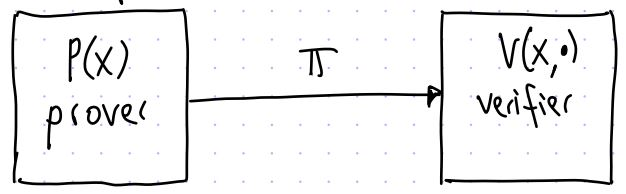
\includegraphics[width=0.6\textwidth]{NP.JPG}
  \caption{$\mathcal{NP}$ Proof Systems}
\end{figure}

\section{Interactive Proofs}

Here is a demonstration of the theorem environments.

\begin{theorem}
This is a theorem.
\end{theorem}

\begin{definition}
This is a definition.
\end{definition}

\begin{remark}
This is a remark.
\end{remark}

\begin{lemma}
This is a lemma.
\end{lemma}

\begin{corollary}
This is a corollary.
\end{corollary}

\begin{proposition}
This is a proposition.
\end{proposition}

\begin{claim}
This is a claim.
\end{claim}

\begin{observation}
This is an observation.
\end{observation}

\begin{fact}
This is a fact.
\end{fact}

\begin{assumption}
This is an assumption.
\end{assumption}

\subsection{Proof Environments}

Here is a demonstration of the proof environments.

\begin{theorem}
\label{thm:thm1}
This is a theorem with a proof.
\end{theorem}

\begin{proof}
This is the theorem's proof.
\end{proof}

\begin{theorem}
This is a theorem with a proof claim.
\end{theorem}

\begin{proof_claim}
This is the theorem's proof claim.
\end{proof_claim}

\begin{proof_of}{Theorem \ref{thm:thm1}}
This is another proof of Theorem \ref{thm:thm1}.
\end{proof_of}


%%%%%%%%%%%%%%%%%%%%%%%%%%%%%%%%%%%%%%%%%%%%%%%%%%%%%%%%%%%%%%%%%%%%%%%%%%%%%%%

% bibliography goes here
\bibliographystyle{amsalpha}

\end{document}
%%%%%%%%%%%%%%%%%%%%%%%%%%%%%%%%%%%%%%%%%%%%%%%%%%%%%%%%%%%%%%%%%%%%%%%%%%%%%%%